\begin{figure}[t]
  \centering
  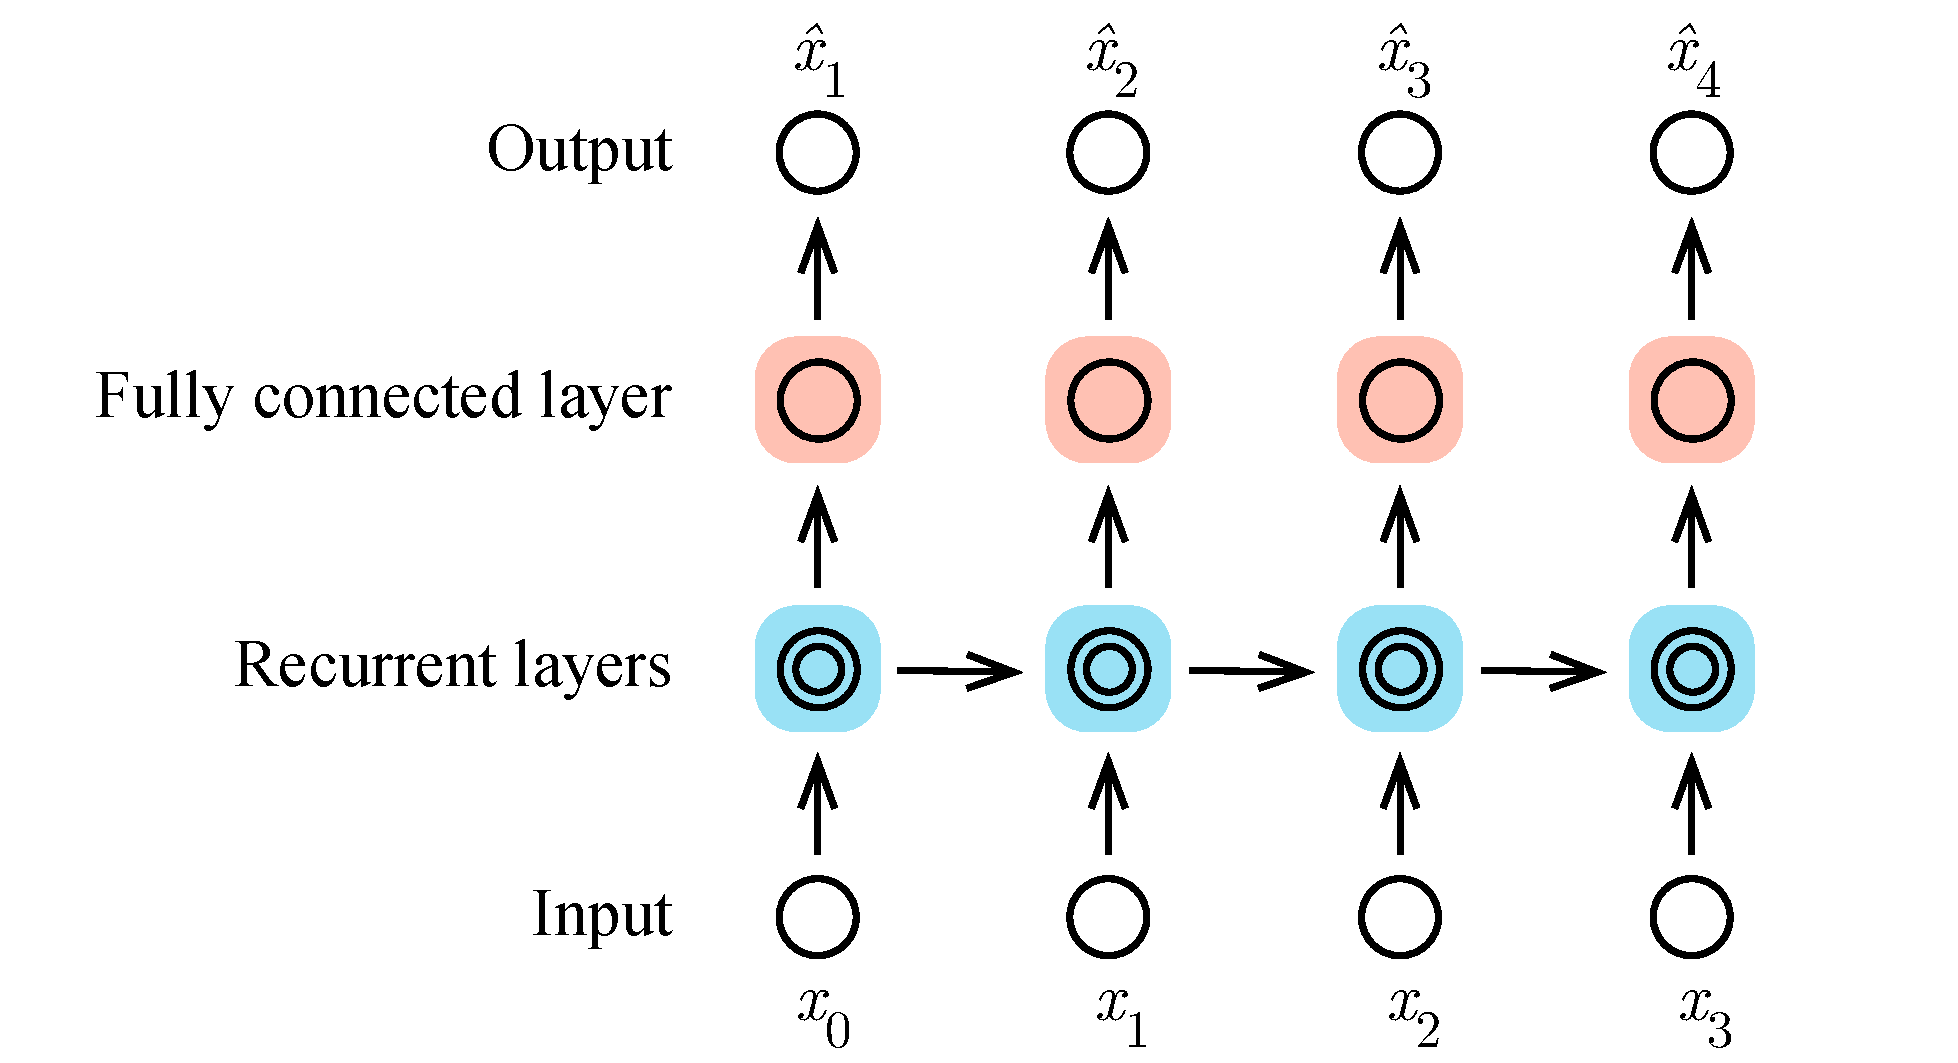
\includegraphics[width=1.0\columnwidth]{include/assets/figures/unroll.pdf}
  \vspace{-1.5em}
  \caption{An example of dynamic unrolling during the model's usage.}
  \vspace{-1.5em}
  \flab{unroll}
\end{figure}

The output of the data-processing stage described in \sref{data} is the data set
$X$, which is split into three catalogs of TFRecord files (for training,
validation, and testing).

\subsection{Training}
In our experiments, we use the Adam optimizer \cite{kingma2014}.

\subsection{Validation}
To this end, we use Hyperband \cite{li2016}.

\subsection{Testing}
In order to have a long-range prediction (multiple steps ahead), we use
refeeding: the predicted value $\hat{x}_{i,k + 1}$ is fed into the model as if
it was the actual resource usage $x_{i,k + 1}$ at step $k + 1$, which is not
yet known at time step $k$. The process continues until all the desired $h$
future values are estimated.
